\section{Altium Designer}
\subsection{LED Driver}
In this project, we will show how to build a simple LED driver circuit. A simple driver
 based on BJT is proposed in this section
\subsubsection{Schematic design}
\textbf{Your image goes here:}
\begin{figure}[h!]
    \centering
    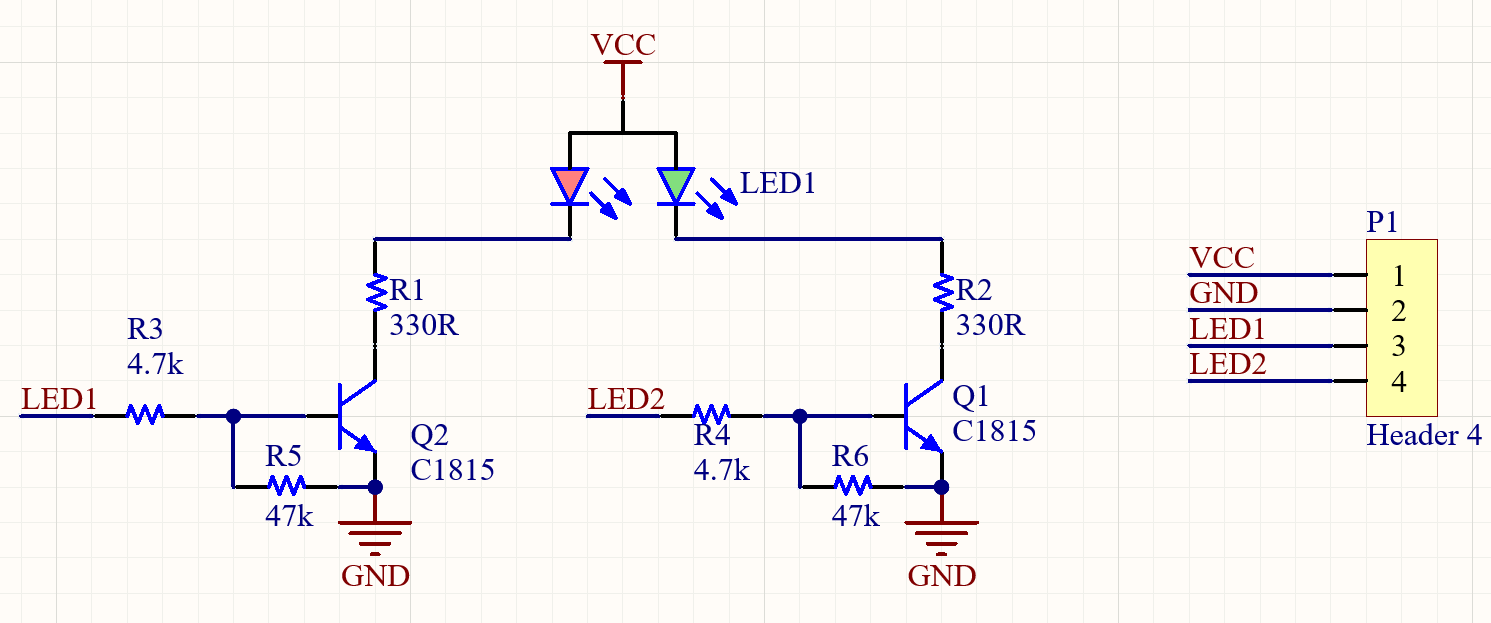
\includegraphics[width=0.89\textwidth]{graphics/ex2/f1.png}
\end{figure}

\subsubsection{PCB layout}

\textbf{Your images go here:}
\begin{figure}[h!]
    \centering
    % Ảnh trái
    \begin{subfigure}{0.495\textwidth}
        \centering
        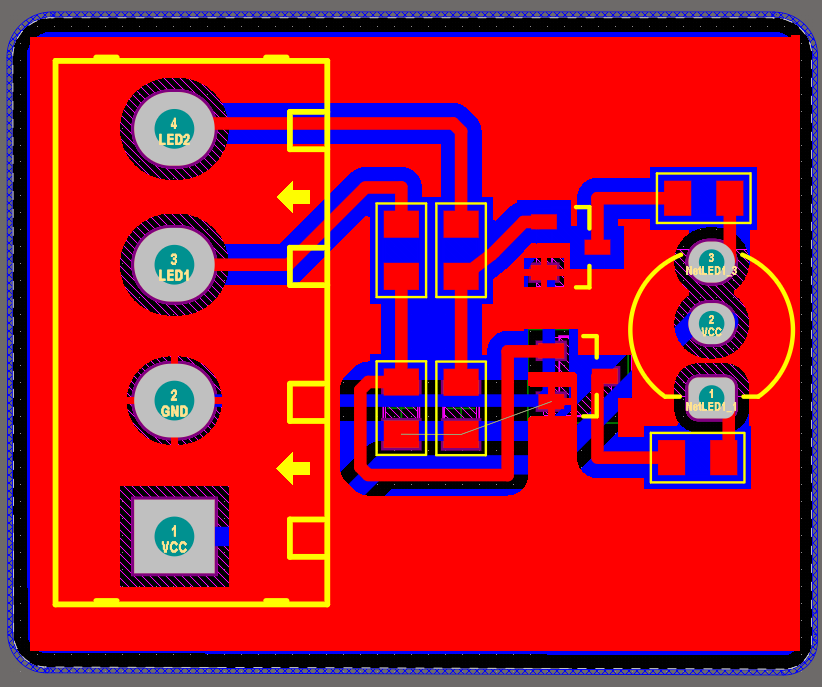
\includegraphics[width=\textwidth]{graphics/ex2/f2.png}
        \caption*{Top Layer}
    \end{subfigure}
    \hfill
    % Ảnh phải
    \begin{subfigure}{0.495\textwidth}
        \centering
        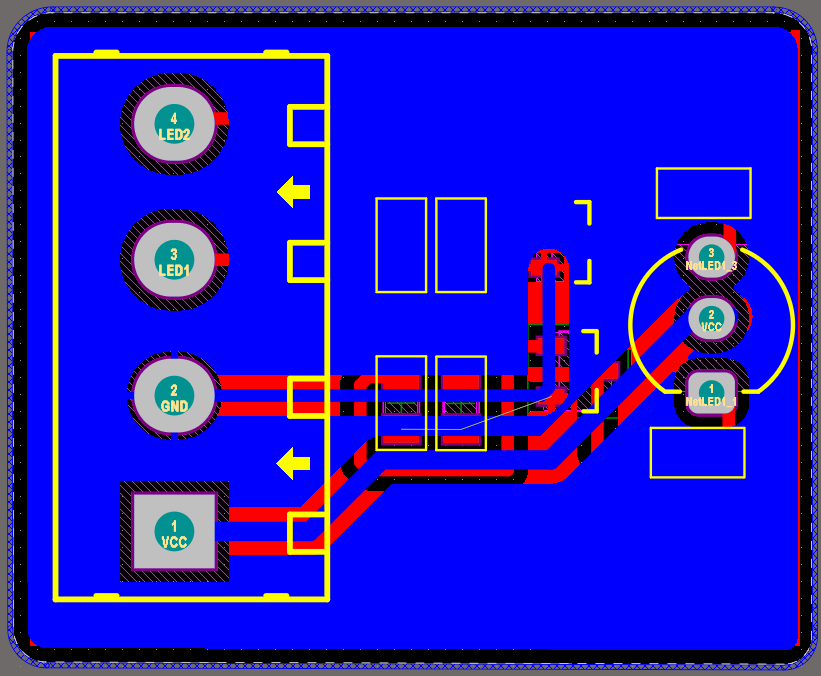
\includegraphics[width=\textwidth]{graphics/ex2/f3.png}
        \caption*{Bottom Layer}
    \end{subfigure}
\end{figure}

\textbf{Some 3D views of the PCB:}
\begin{figure}[h!]
    \centering
    % Ảnh trái
    \begin{subfigure}{0.495\textwidth}
        \centering
        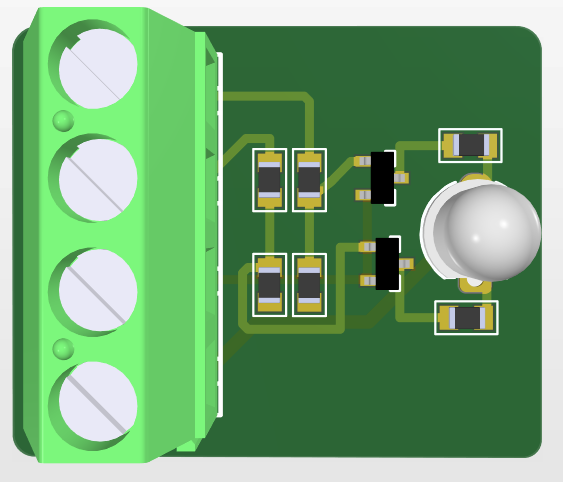
\includegraphics[width=0.95\textwidth]{graphics/ex2/f4.png}
        \caption*{Top view}
    \end{subfigure}
    \hfill
    % Ảnh phải
    \begin{subfigure}{0.495\textwidth}
        \centering
        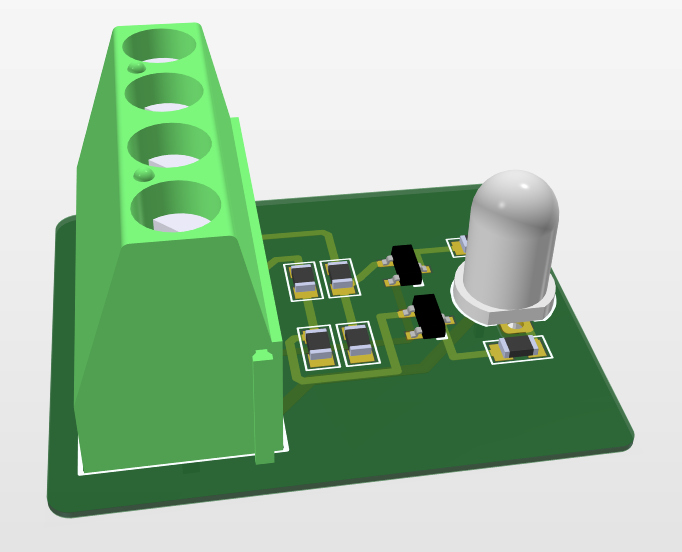
\includegraphics[width=\textwidth]{graphics/ex2/f5.png}
        \caption*{Beside view}
    \end{subfigure}
\end{figure}

\subsection{Relay Controller}
\subsubsection{Schematic design}
\textbf{Your image goes here:}
\begin{figure}[h!]
    \centering
    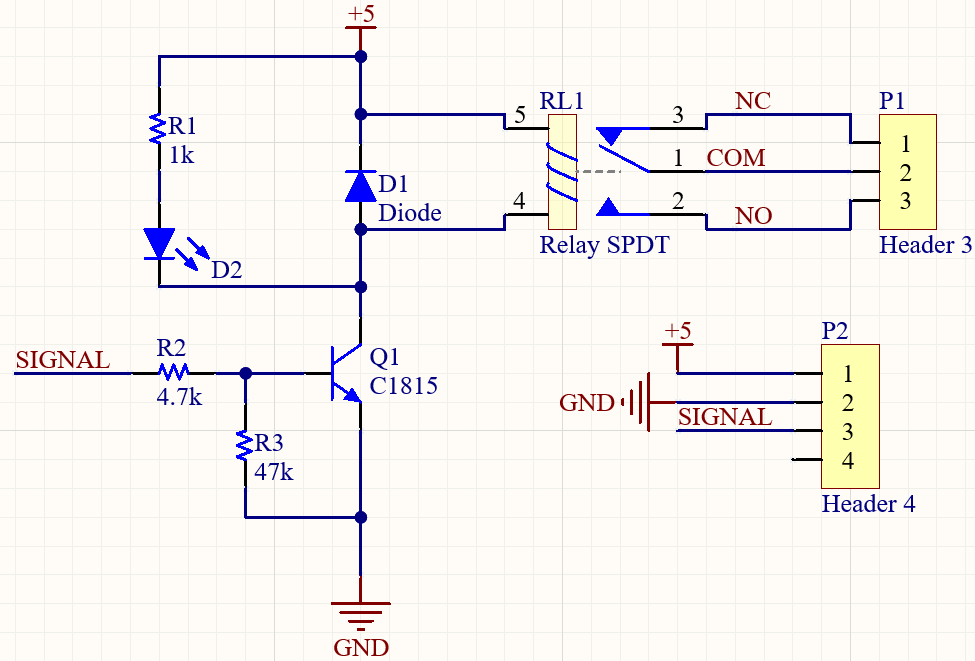
\includegraphics[width=0.8\textwidth]{graphics/ex2/f6.png}
\end{figure}

\subsubsection{PCB layout}
\textbf{Your images go here:}
\begin{figure}[h!]
    \centering
    % Ảnh trái
    \begin{subfigure}{0.495\textwidth}
        \centering
        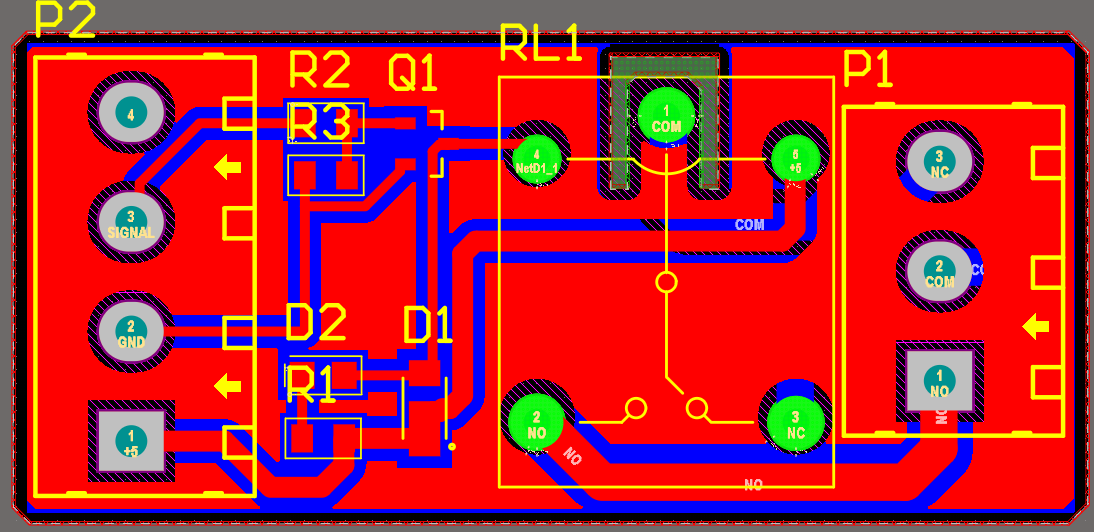
\includegraphics[width=\textwidth]{graphics/ex2/f7.png}
        \caption*{Top Layer}
    \end{subfigure}
    \hfill
    % Ảnh phải
    \begin{subfigure}{0.495\textwidth}
        \centering
        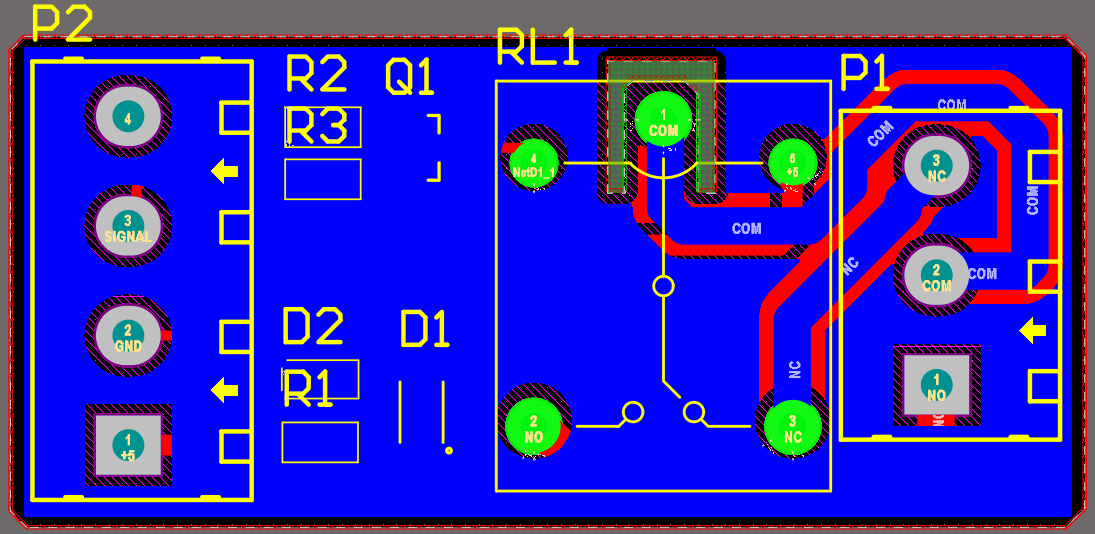
\includegraphics[width=\textwidth]{graphics/ex2/f8.png}
        \caption*{Bottom Layer}
    \end{subfigure}
\end{figure}

\textbf{Some 3D views of the PCB:}
\begin{figure}[h!]
    \centering
    % Ảnh trái
    \begin{subfigure}{0.495\textwidth}
        \centering
        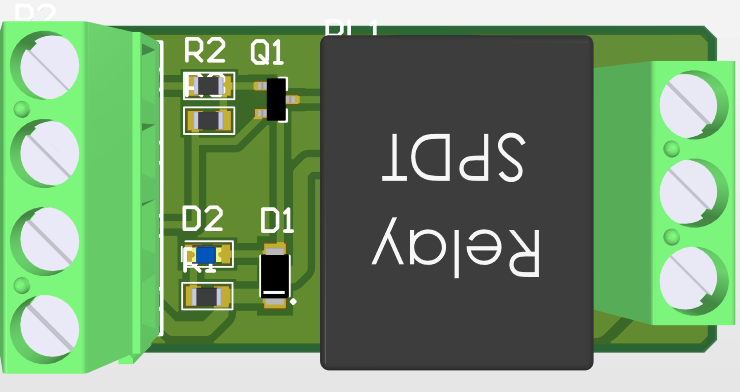
\includegraphics[width=0.95\textwidth]{graphics/ex2/f9.png}
        \caption*{Top-down view}
    \end{subfigure}
    \hfill
    % Ảnh phải
    \begin{subfigure}{0.495\textwidth}
        \centering
        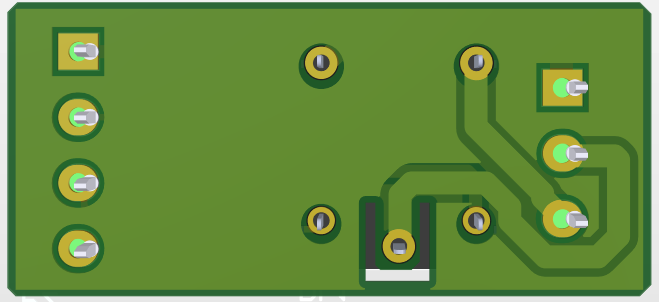
\includegraphics[width=\textwidth]{graphics/ex2/f10.png}
        \caption*{Bottom-up view}
    \end{subfigure}
\end{figure}